\documentclass[a4paper,11pt]{article}

\usepackage{mlsubmit,amsmath, algorithm}
\usepackage{algpseudocode}
\usepackage{algorithmic}




\begin{document}

\initmlsubmision{2} % assignment number
{Piyush Bagad}   % your name
{150487}	% your roll number

\begin{mlsolution}
Consider a logistic regression model with gaussian prior.
\[
p(y_n | \vec{x_n}, \vec{w}) = \frac{1}{1+\exp(-y_n \vec{w}^T\vec{x_n})}, \ \ p(\vec{w}) = \mathcal{N}(\vec{0}, \lambda^{-1}\vec{I})
\]
For MAP estimation, we need to solve the following maximization problem:
\[
\vec{\hat{w}}_{MAP} = \arg \min_{w} \mathcal{L}(\vec{w})=  \arg \min_{w} \left( -\sum_{n=1}^{N}\log(p(y_n| \vec{x_n}, \vec{w}))  - log(p(\vec{w}))\right) 
\]
\[
\log(p(y_n| \vec{x_n}, \vec{w})) = - \log(1 + \exp(-y_n \vec{w}^T\vec{x_n}), \ \ \log(p(\vec{w})) = -(D/2)\log(2\pi) + \log(\lambda) - (\lambda/2)\vec{w}^{T}\vec{w}
\]
\[
\therefore \mathcal{L}(\vec{w}) = \sum_{n=1}^{N}\log(1 + \exp(-y_n \vec{w}^T\vec{x_n}) + \frac{\lambda}{2}\vec{w}^{T}\vec{w}
\]
Computing the partial derivative w.r.t $\vec{w}$ , and equating to 0, we get
\[
\frac{\partial \mathcal{L}}{\partial \vec{w}} = \sum_{n=1}^{N}\frac{-y_n \vec{x}_n}{1 + \exp(-y_n \vec{w}^T\vec{x_n})} + \lambda\vec{w} \Rightarrow \boxed{\vec{w} = \sum_{n=1}^{N}y_n\alpha_n \vec{x}_n}
\]
\[
\text{where} \ \  \alpha_n(\vec{w}) = \frac{1}{\lambda(1 + \exp(-y_n \vec{w}^T\vec{x_n}))} = \frac{p(y_n | \vec{x}_n, \vec{w})}{\lambda}
\]
Thus, the MAP estimate is trying to weigh examples based on the prediction probability of each given example. It will ignore the examples on which the predicted probability is low $(p(y_n|\vec{x_n}, \vec{w}) \rightarrow 0)$ and consider only those examples that have this predicted probability high much like the support vectors in SVM. The hyperparamter $\lambda$ will decide the amount of regularization as usual.  

\end{mlsolution}

\begin{mlsolution} 
Consider a generative classification model for binary classification with the Naive Bayes assumption of feature independence. Let the class marginal and class conditional distributions be as follows:
\[
p(y = 1) = \pi, \ \ p(\vec{x}| y = j) = \prod_{d=1}^{D}\text{Bernoulli}(x_d | \mu_{d,j}) = \prod_{d=1}^{D} \mu_{d,j}^{x_d}(1- \mu_{d,j})^{1-x_d}, \ \ j = 0,1
\]
For convenience, let us consider simplification of only $p(y = 1 | \vec{x})$.
\[
p(y = 1 | \vec{x}) = \frac{p(\vec{x} | y = 1)p(y=1)}{p(\vec{x})} = \frac{p(\vec{x} | y = 1)p(y=1)}{p(\vec{x} | y = 1)p(y=1) + p(\vec{x} | y = 0)p(y=0)}
\]
\[
\therefore p(y = 1 | \vec{x}) = \frac{\pi \prod_{d=1}^{D} B(x_d, \mu_{d,1})}{\pi \prod_{d=1}^{D}B(x_d, \mu_{d,1}) + (1- \pi) \prod_{d=1}^{D}B(x_d, \mu_{d,0})}; \ \ \ \text{where} \ \ B \ \ \text{denotes Bernoulli}
\]
\[
\therefore p(y = 1 | \vec{x}) = \frac{1}{1 + \frac{1-\pi}{\pi}\frac{\prod_{d=1}^{D}B(x_d, \mu_{d,1})}{\prod_{d=1}^{D}B(x_d, \mu_{d,0})}} = \frac{1}{1 + \frac{1-\pi}{\pi}\prod_{d=1}^{D}(\frac{\mu_{d0}}{\mu_{d1}})^{x_d}(\frac{1-\mu_{d0}}{1-\mu_{d1}})^{1-x_d}}
\]
Now, let $s_d = \frac{\mu_{d0}}{\mu_{d1}}$, $r_d = \frac{1-\mu_{d0}}{1-\mu_{d1}}$ and $C = \frac{1-\pi}{\pi}$. On further simplifying, we get
\[
p(y=1|\vec{x}) = \frac{1}{1 + C\prod_{d=1}^{D}s_{d}^{x_d}r_{d}^{1-x_d}} = \frac{1}{1 + \exp\left( \log(C) + \sum_{d=1}^{D}x_d\log(s_d) + (1-x_d)\log(r_d)\right) }
\]
\[
\therefore \boxed{p(y=1|\vec{x}) = \frac{1}{1 + \exp(\vec{w}^{T}\vec{x} + b)}}  
\]
\[
\text{where} \ \ \vec{w} = [\log(s_1)-\log(r_1),...,\log(s_D)-\log(r_D)]^{T} \text{and} \  b = \log\left( C(\prod_{d=1}^{D}r_d)\right) 
\]
Thus, this corresponds to the discriminative logistic regression model for binary classification with  labels $\in \{0,1\}$. The decision boundary is linear.


\end{mlsolution}

\begin{mlsolution}
Consider the following constrained version of least squares linear regression:
\[
\vec{\hat{w}} = \arg\min_{w} \sum_{n=1}^{N}\left( y_n - \vec{w}^{T}\vec{x}_n \right) ^{2} \ \ \text{subject to} \ \ \Vert\vec{w}\Vert \leq c
\]
Note that the constraint $\Vert\vec{w}\Vert \leq c$ is equivalent to $\Vert\vec{w}\Vert^{2} \leq c^{2}$ since $\Vert\vec{w}\Vert \geq 0$.
The lagrangian function for the modified constrained problem can be stated as:
\[
\mathcal{L}(\vec{w}, \alpha) = \sum_{n=1}^{N}\left( y_n - \vec{w}^{T}\vec{x}_n \right) ^{2} + \alpha(\Vert\vec{w}\Vert^{2} - c^2)
\]
Ignoring the constant and re-writing,
\[
\mathcal{L}(\vec{w}, \alpha) = \sum_{n=1}^{N}\left( y_n - \vec{w}^{T}\vec{x}_n \right) ^{2} + \alpha\vec{w}^{T}\vec{w} = (\vec{y} - \vec{X}\vec{w})^{T}(\vec{y} - \vec{X}\vec{w}) + \alpha \vec{w}^{T}\vec{w}
\]
Solving using the dual variable technique (We can do it since both the objective and constraint are convex),
\[
\frac{\partial \mathcal{L}}{\partial \vec{w}} = -2\vec{X}^{T}\vec{y} + 2(\vec{X}^T\vec{X} + \alpha \vec{I})\vec{w} = 0
\]
\[
\boxed{\vec{w} = \left( \vec{X}^T\vec{X} + \alpha \vec{I} \right) ^{-1}\vec{X}^{T}\vec{y}}
\]
\[
\therefore \mathcal{L}_D(\alpha) = \vec{y}^T\vec{y} - \vec{w}^T\vec{X}^{T}y - \vec{y}^{T}\vec{X}\vec{w} + \vec{w}^{T}(\vec{X}^{T}\vec{X}+\alpha\vec{I})\vec{w}
\]
\[
\therefore \mathcal{L}_D(\alpha) = \vec{y}^T\vec{y} - \vec{w}^T\vec{X}^{T}y - \vec{y}^{T}\vec{X}\vec{w} + \vec{w}^{T}\vec{X}^{T}\vec{y} = \vec{y}^T\vec{y} - \vec{y}^{T}\vec{X}\vec{w}
\]
Ignoring the term $\vec{y}^T\vec{y}$, we get
\[
\mathcal{L}_D(\alpha) = -\vec{y}^{T}\vec{X}\vec{w} = - (\vec{X}^T\vec{y})^{T}\left(  \vec{X}^T\vec{X} + \alpha \vec{I} \right)^{-1}\vec{X}^{T}\vec{y} = -\vec{Z}^{T}\vec{M}^{-1}_\alpha\vec{Z}
\]
\[
\frac{\partial \mathcal{L}}{\partial \alpha} = -\frac{\partial [\vec{Z}^{T}\vec{M}^{-1}_\alpha\vec{Z}]}{\partial \vec{M}_\alpha}\frac{\partial \vec{M}_\alpha}{\partial \alpha} = (\vec{M}^{-1}_\alpha\vec{Z}\vec{Z}^{T}\vec{M}^{-1}_\alpha)^{-1}\vec{I}
\]
\[
\therefore \frac{\partial \mathcal{L}}{\partial \alpha} = (\vec{M}^{-1}_\alpha \vec{X}^{T}\vec{y}\vec{y}^{T}\vec{X} \vec{M}^{-1}_\alpha)^{-1}
\]
Note that $\vec{M}^{T}_\alpha = \vec{M}_\alpha$ and thus we have
\[
\therefore \frac{\partial \mathcal{L}}{\partial \alpha} = ((\vec{M}^{-1}_\alpha \vec{X}^{T}\vec{y})(\vec{M}^{-1}_\alpha \vec{X}^{T}\vec{y})^{T})^{-1}
\]
\end{mlsolution}

\begin{mlsolution}
Consider $N$ training examples $\{x_n , y_n \}^{N}_{n=1}$ where $x_n \in \mathbb{R}^{D}, y_n \in \mathbb{R}^{K}$. Consider the softmax regression model for multi-class classification:
\[
p(y_n = k| x_n, W) = \mu_{nk} = \frac{\exp(w^{T}_{k}x_n)}{\sum_{l=1}^{K}\exp(w^{T}_{l}x_n)}
\]
The MLE objective can be stated as: $\hat{W}_{MLE} = \arg \min_{W} - NLL(W)$. Let us work for each column $w_k$ of $W$:
\[
\frac{-\partial NLL(W)}{\partial w_k} = -\sum_{n=1}^{N}\frac{ \partial\log(p(y_n=k|x_n,W))}{\partial w_k}
\]
\[
\log(p(y_n=k|x_n,W)) = w^{T}_k x_n - \log\left( \sum_{l=1}^{K}\exp(w^{T}_l x_n) \right) 
\]
\[
\therefore \frac{ \partial\log(p(y_n=k|x_n,W))}{\partial w_k} = x_n - \mu_{nk}x_n
\]
\[
\therefore \frac{-\partial NLL(W)}{\partial w_k} = \sum_{n=1}^{N}x_n(\mu_{nk}-1) = X^{T}\text{Diagonal}([\mu_{1k}-1, \mu_{2k}-1,..,\mu_{Nk}-1])
\]
Thus, no closed form solution for $w_k$ can be computed from this equation. We can write the gradient descent update for $w_k$ with $\eta = 1$ as follows:
\[
\boxed{w^{(t+1)}_{k} = w^{(t)}_{k} - \sum_{n=1}^{N}x_n\left( \mu^{(t)}_{nk}-1\right) }
\]
Similarly, the stochastic gradient descent update will turn out to be:
\[
\boxed{w^{(t+1)}_{k} = w^{(t)}_{k} - x_n(\mu^{(t)}_{nk}-1) }
\]
Consider the case of 'hard' assignments i.e. let $k = \arg \max_{k} \mu_{nk}$ and $\mu_{nk'} = 0, \forall k' \neq k$. The SGD update will simple reduce to 
\[
w^{(t+1)}_{k} = w^{(t)}_{k} - x_n(\mu^{(t)}_{nk}-1) =
\begin{cases}
w^{(t)}_{k} & \text{for }p(y_n=k|x_n, W) = 1\\    
w^{(t)}_{k} + x_n  & \text{for }p(y_n=k|x_n, W) = 0
\end{cases}
\]
Thus, we simply do NOT update the weight vector $w_k$ if we encounter an example $(x_n, y_n)$ such that the current prediction  is correct i.e. whose label is $k$. Else, we make the weight vector $w_k$ move in the direction of $x_n$. The SGD algorithm sketch for this case will be as follows:

\begin{algorithm}
	\caption{Multi-class Stochastic Gradient Descent}\label{alg:gibbs}
	\begin{algorithmic}[5]
		\State Choose initial $w_k = w^{(0)}_k, \forall k \in \{1,2,..K\}$.
		\For{$k \in \{1,2,..K\}$ }
		\State $\#$ Keeping $w_{l}, \  \text{for}\ \  l \neq k$ fixed, update $w_k$
		\For{$s$ iterations until convergence}
		\If{$p(y_n| x_n, W^{(t)}) = 1$}
		\State $w^{(t+1)}_k = w^{(t)}_k$
		\Else
		\State $w^{(t+1)}_k = w^{(t)}_k + x_n$
		\EndIf
		\EndFor
		\EndFor
	\end{algorithmic}
\end{algorithm}

\end{mlsolution}
	
\begin{mlsolution}

Let $C_x$ and $C_y$ be the convex hulls corresponding to points $X = \{\vec{x}_i\}^{N}_{i=1}$ and $Y = \{\vec{y}_i\}^{N}_{i=1}$ respectively. 
\[
C_X := \{  x = \sum_{n=1}^{N}\alpha_n x_n \ : \ \alpha_i \geq 0, \sum_{i}\alpha_i = 1 \}
\]
\vspace{-2mm}
\[
C_Y := \{  x = \sum_{n=1}^{N}\beta_n y_n \ : \ \beta_i \geq 0, \sum_{i}\beta_i = 1 \}
\]

\begin{definition}
	\label{lin_sep}
	The sets of points $X$ and $Y$ are said to be linearly seperable if $\exists$ a line (hyperplane in high dimensional space) $L := \{ \vec{x}\in \mathbb{R}^{D} : \ m^{T}\vec{x} + b = 0 \}$ such that $m^{T}\vec{x}_i + b \geq 0, \text{and} \  m^{T}\vec{y}_i + b < 0 \ \forall \ i = 1,2,..N$.
\end{definition}
We have to show that $X$ and $Y$ are linearly separable \textit{iff} $C_X \cap C_Y = \phi$ \\

$(\Rightarrow)$ Assume that $X$ and $Y$ are linearly separable. Suppose for contradiction that $C_X \cap C_Y \neq \phi$. This implies that $\exists z \in C_X \cap C_Y$. Thus, by definition, 
\[
z = \sum_{n=1}^{N}\alpha_n x_n \ = \sum_{n=1}^{N}\beta_n y_n \
\]
where $\alpha_i \geq 0, \sum_{i}\alpha_i = 1, \beta_i \geq 0, \sum_{i}\beta_i = 1$. Since, $X$ and $Y$ are linearly separable, there exists a line $L$ satisfying $m^{T}\vec{x}_i + b \geq 0, \text{and} \  m^{T}\vec{y}_i + b < 0 \ \forall \ i = 1,2,..N$.  Now, since $\alpha_i \geq 0, \forall i$, 
\[
\alpha_im^{T}\vec{x}_i + \alpha_ib \geq 0, \forall i = 1,2,..,N
\]
\begin{equation}
\label{eq1}
\therefore \sum_{n=1}^{N} \alpha_n m^{T}\vec{x}_n + \sum_{n=1}^{N}\alpha_i b = \sum_{n=1}^{N} \alpha_n m^{T}\vec{x}_n + b.1 = m^{T}z + b \geq 0
\end{equation}
Similarly, since $\beta_im^{T}\vec{y}_i + \beta_ib < 0 \ \forall \ i = 1,2,..N$,
\begin{equation}
\label{eq2}
\therefore \sum_{n=1}^{N} \beta_n m^{T}\vec{x}_n + \sum_{n=1}^{N}\beta_n b = \sum_{n=1}^{N} \beta_n m^{T}\vec{x}_n + b.1 = m^{T}z + b < 0
\end{equation}
The equations \ref{eq1} and \ref{eq2} present a contradiction. Thus, we have $C_X \cap C_Y = \phi$.\\

$(\Leftarrow)$ To show the converse, assume that $C_X \cap C_Y = \phi$. To show that $X$ and $Y$ are linearly separable i.e. we have to find $L$ satisfying definition \ref{lin_sep}. Define
\[
d := \min_{x \in C_X ,y \in C_Y}\Vert x - y \Vert^{2}
\]
Note, since $C_X$ and $C_Y$ are closed and bounded, the quantity $d$ exists and suppose it achieves the minima at $x_o \in C_X, y_o \in C_Y$ .Also $d>0$ since $C_X \cap C_Y = \phi$. Let $L$ be the perpendicular bisector of the line joining $x_o$ and $y_o$.  It is trivial to observe that $L$ is a linear separator of $X$ and $Y$. Hence, we are done.


\end{mlsolution}

\begin{mlsolution}

The original hard-margin SVM optimization problem can be stated as
\begin{gather*}
\arg \min_{w,b} \frac{\Vert w \Vert^{2}}{2} \\
\text{subject to} \ \ \  y_n(w^{T}x_n + b)\geq 1, \ \ \forall \ n = 1,2,..,N
\end{gather*}
The modified version of SVM involves changing the inequalities as  $y_n(w^{T}x_n + b)\geq m, \ \ \forall \ n = 1,2,..,N$. Let $\mathbf{\alpha} = [\alpha_1, \alpha_2,..,\alpha_N]$ be the lagrange variables. The lagrangian can be stated as
\[
\mathcal{L}(w,b, \mathbf{\alpha}) = \frac{\Vert w \Vert^{2}}{2} + \sum^{N}_{n=1}\alpha_n(m - y_n(w^{T}x_n + b))
\]
Using the dual formulation to solve for the constrained optimization problem, we have
\[
 \frac{\partial \mathcal{L}(w, \mathbf{\alpha})}{\partial w} = 0 \Rightarrow \boxed{w = \sum^{N}_{n=1}\alpha_n y_nx_n}, \ \frac{\partial \mathcal{L}(w, \mathbf{\alpha})}{\partial b} = 0 \Rightarrow \boxed{\sum^{N}_{n=1}\alpha_n y_n = 0}
\] 
Now, Substituting $w = \sum^{N}_{n=1}\alpha_n y_nx_n$ in Lagrangian, we get the dual problem as 
\[
\mathcal{L}_D(\mathbf{\alpha}) = w^{T}w + \sum^{N}_{n=1}(\alpha_n m - y_n b) - \sum^{N}_{n=1}y_n w^{T}x_n = \sum^{N}_{n=1}\alpha_n m - \frac{1}{2} \sum_{n,l =1}^{N}\alpha_l \alpha_n y_l y_n (x^{T}_l x_{n})
\]
Now, the objective can be stated in a compact form as
\[
\max_{\alpha \geq 0} \  m(\alpha^{T}\vec{1}) - \frac{1}{2}\alpha^{T}G \alpha  
\]
where G is an $N\times N$ matrix with $G_{ln} = y_l y_n x^{T}_l x_n$, and $\vec{1}$ is a vector of 1s. Note that $m$ simply turns out to be a mutiplicative constant and thus does not affect the solution of the optimization problem. Thus, the solution to modified SVM effectively remains the same as that of original one.

\end{mlsolution}

\begin{mlsolution}

\section{Part 1: Dataset - \texttt{binclass.txt}}
\label{dataset1}
\subsection{1a: Modeling positive and negative classes with different covariances}
In this case, we assume that the positively labeled examples are sampled from the gaussian $\mathcal{N}(\vec{x}| \mu_{+}, \sigma^{2}_{+}\vec{I})$ and the negatively labeled examples from $\mathcal{N}(\vec{x}|  \mu_{-}, \sigma^{2}_{-}\vec{I})$. Refer to figure \ref{gc1a}. Notice the non linearlity of the decision boundary.

\begin{figure}[!htb]
	\centering
	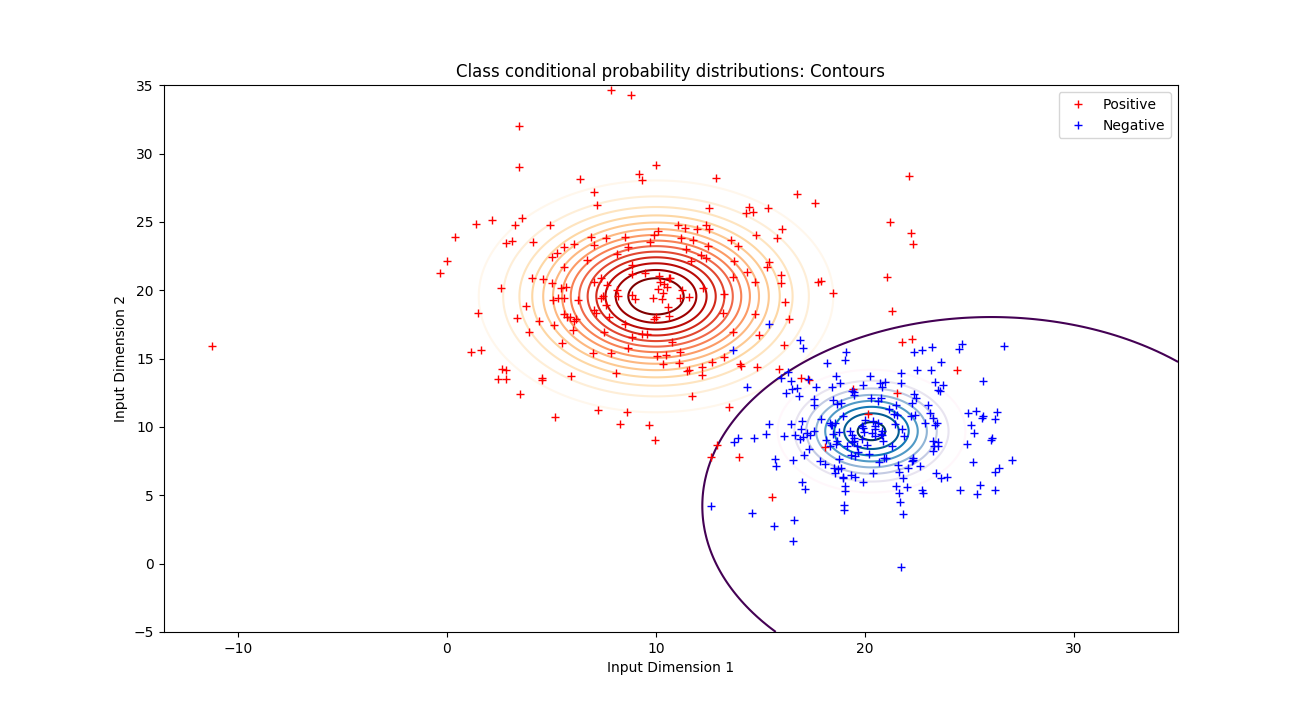
\includegraphics[scale=0.4]{generative_binclass.png}
	\caption{Decision boundary learned by generative classification with gaussian class conditional distributions having different covariances.}
	\label{gc1a}
\end{figure}


\subsection{1b: Modeling positive and negative classes with same covariances}
In this case, we assume that the positively labeled examples are sampled from the gaussian $\mathcal{N}(\vec{x}| \mu_{+}, \sigma^{2}\vec{I})$ and the negatively labeled examples from $\mathcal{N}(\vec{x}|  \mu_{-}, \sigma^{2}\vec{I})$. Note that the covariance matrices for each of the two distributions is the same. Refer to figure \ref{gc1b}. Notice the linearlity of the decision boundary.

\begin{figure}[!htb]
	\centering
	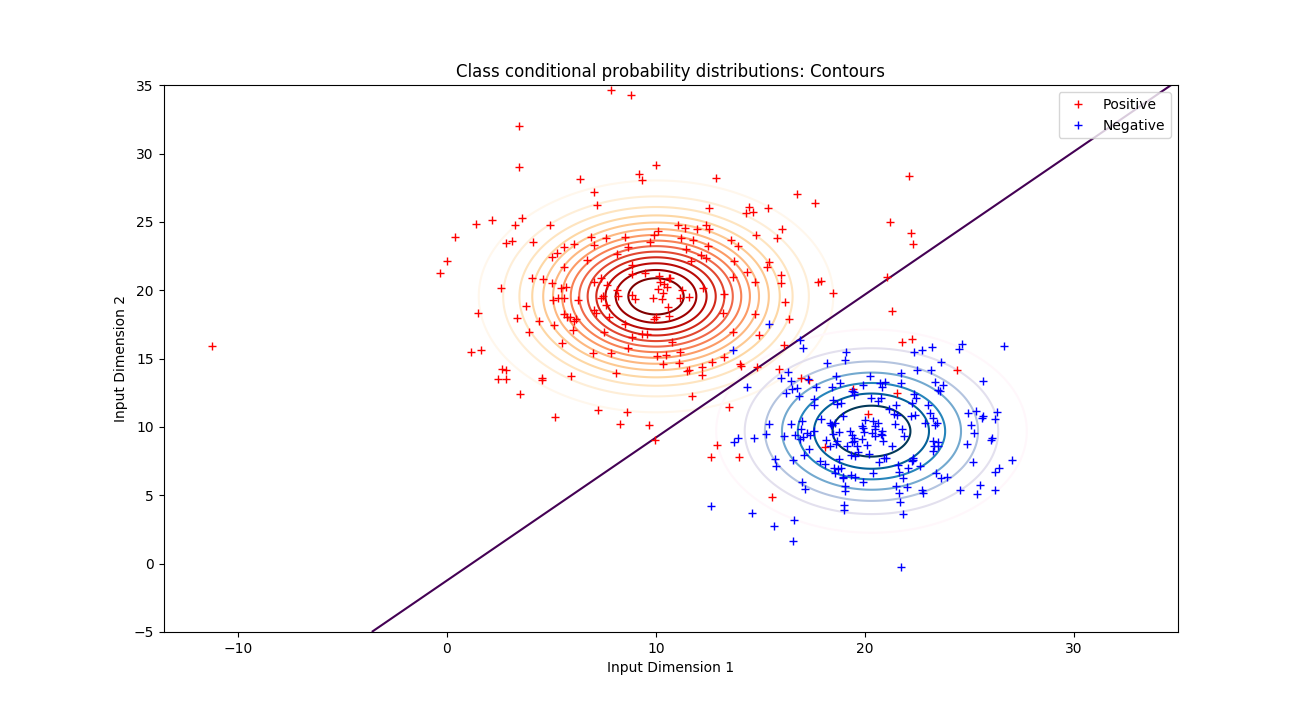
\includegraphics[scale=0.4]{generative_same_covariance_binclass.png}
	\caption{(Linear) Decision boundary learned by generative classification with gaussian class conditional distributions having same covariances.}
	\label{gc1b}
\end{figure}

\subsection{1c: Linear SVM Decision Boundary}
I have used \texttt{linearSVC} library from the \texttt{sklearn.svm} package (\href{http://scikit-learn.org/stable/modules/generated/sklearn.svm.LinearSVC.html}{link}). Refer to figure \ref{svm1}.
\begin{figure}[!htb]
	\centering
	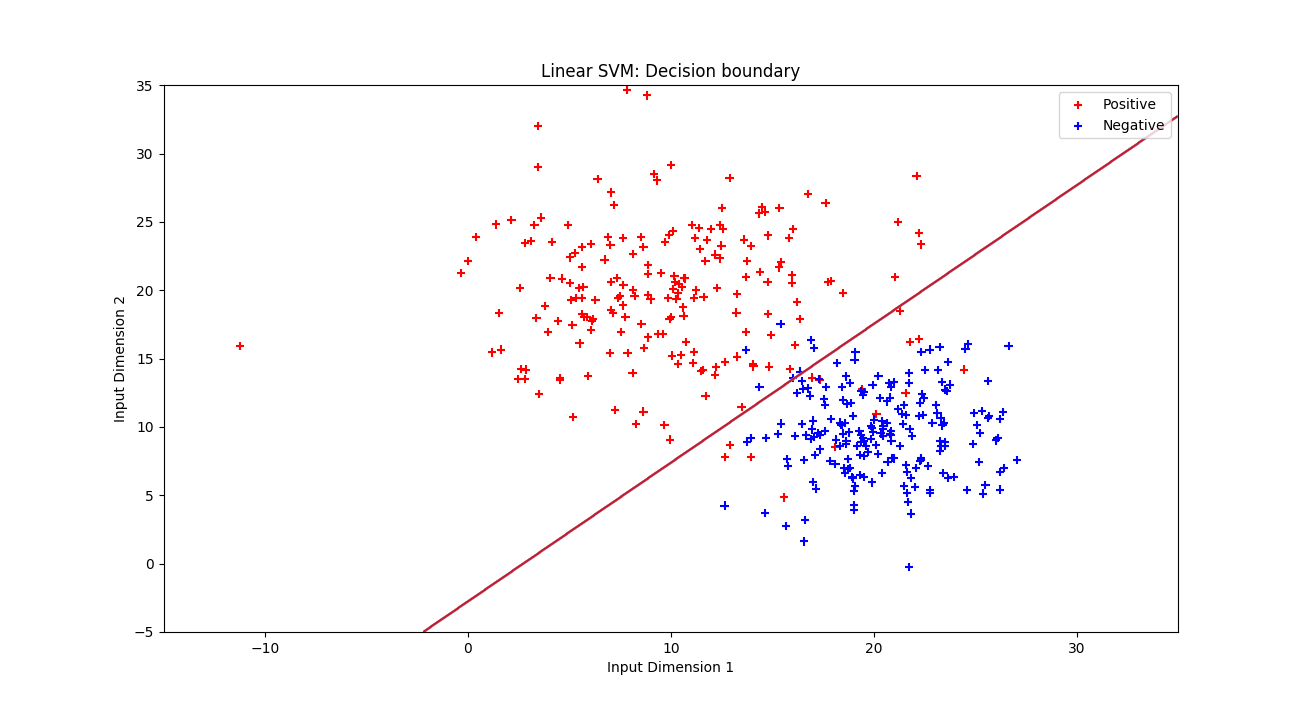
\includegraphics[scale=0.4]{linear_svm_binclass.png}
	\caption{Decision boundary learned by Linear SVM using \texttt{linearSVC} from \texttt{sklearn.svm}.}
	\label{svm1}
\end{figure}

\newpage
\section{Part 2: Dataset - \texttt{binclassv2.txt}}
The experiments corresponding to various subsections for Part \ref{dataset1} have been repeated on the \texttt{binclassv2.txt} dataset and the results are noted below.

\subsection{2a: Modeling positive and negative classes with different covariances}
Refer to figure \ref{gc2a}. Notice the non linearlity of the decision boundary.
\begin{figure}[!htb]
	\centering
	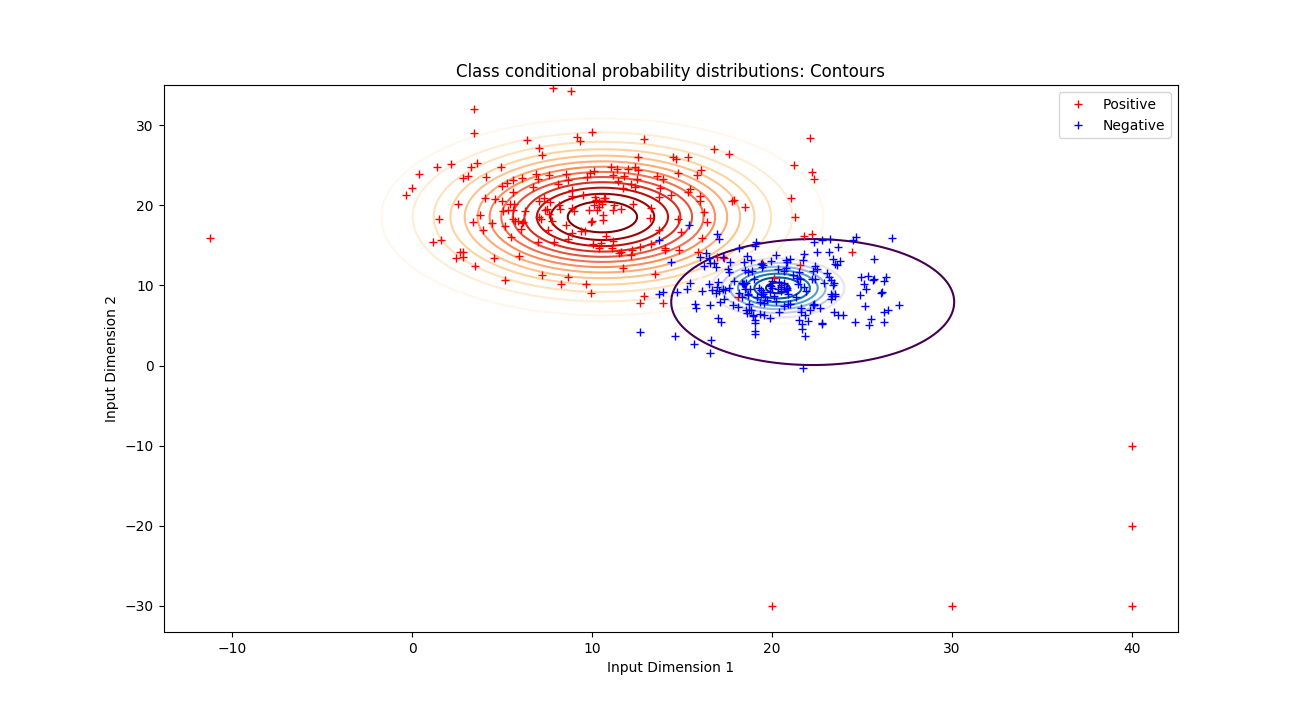
\includegraphics[scale=0.4]{generative_binclassv2.png}
	\caption{Decision boundary learned by generative classification with gaussian class conditional distributions having different covariances.}
	\label{gc2a}
\end{figure}

\subsection{2b: Modeling positive and negative classes with same covariances}
Refer to figure \ref{gc2b}. Notice the linearlity of the decision boundary.
\begin{figure}[!htb]
	\centering
	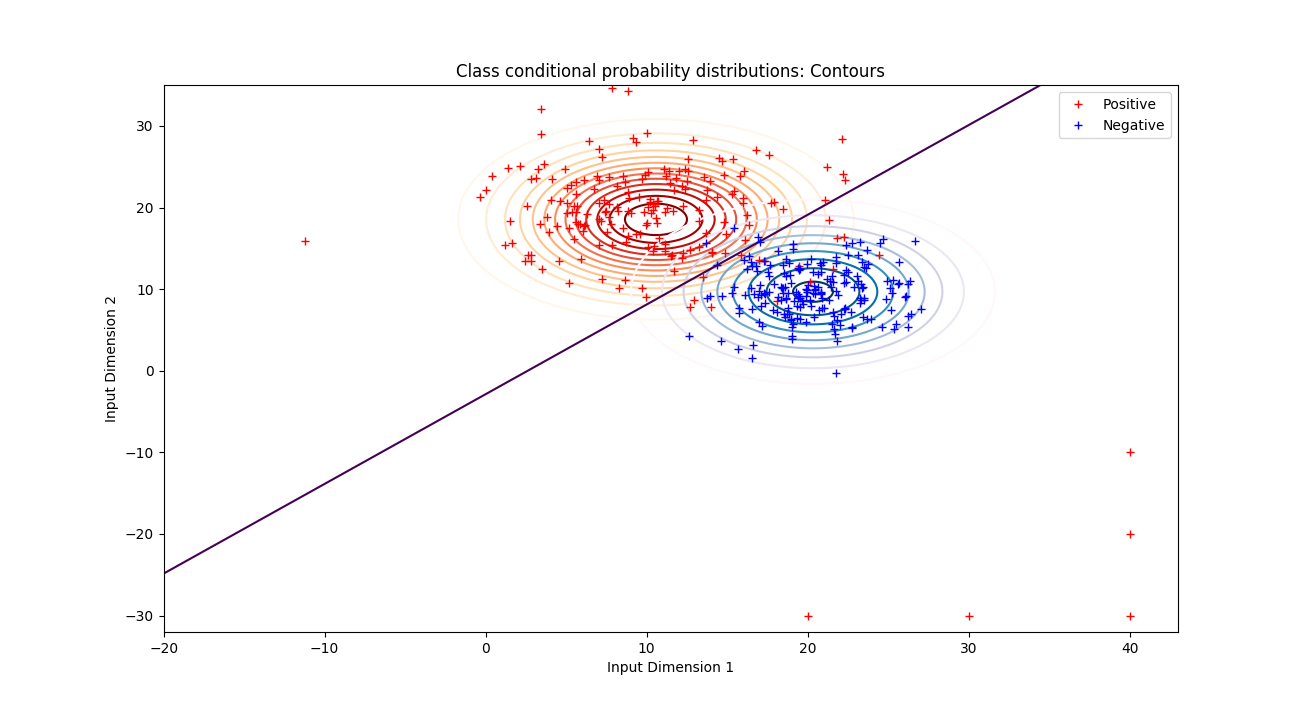
\includegraphics[scale=0.4]{generative_same_covariance_binclassv2.png}
	\caption{(Linear) Decision boundary learned by generative classification with gaussian class conditional distributions having same covariances.}
	\label{gc2b}
\end{figure}


\subsection{2c: Linear SVM Decision Boundary}
Refer to figure \ref{svm2}.
\begin{figure}[!htb]
	\centering
	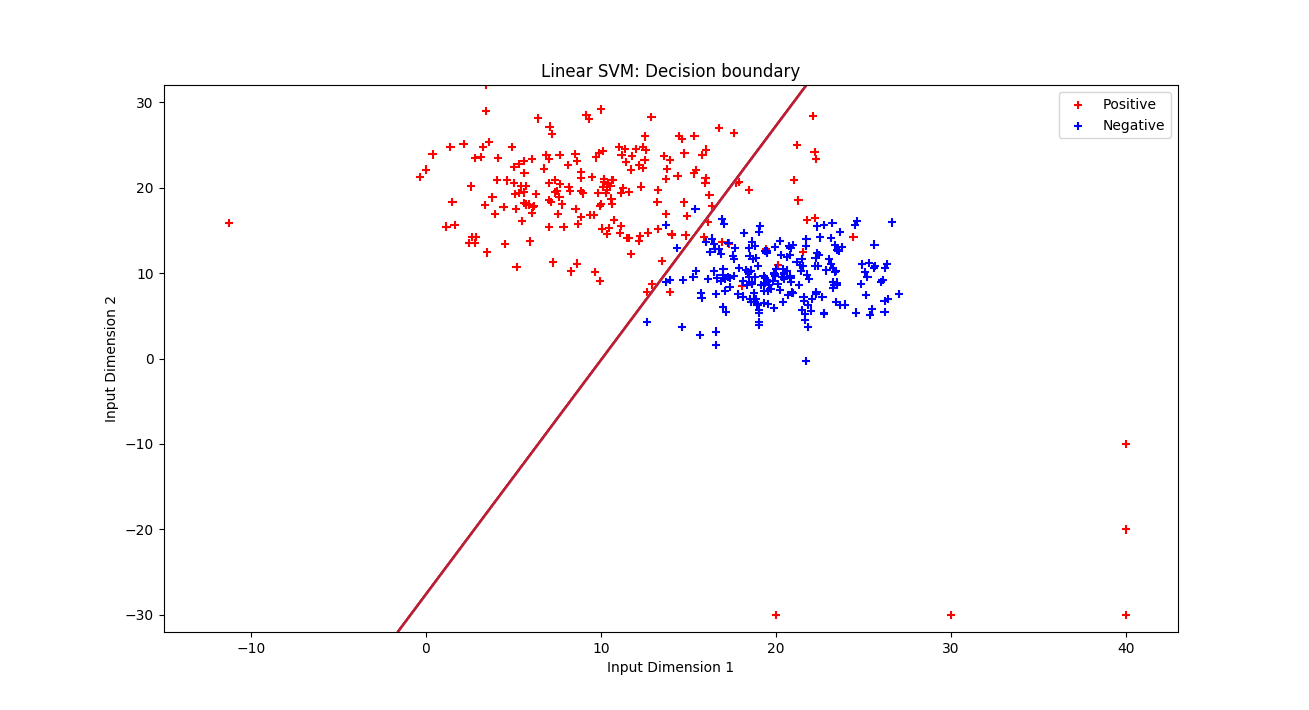
\includegraphics[scale=0.4]{linear_svm_binclassv2.png}
	\caption{Decision boundary learned by Linear SVM using \texttt{linearSVC} from \texttt{sklearn.svm}.}
	\label{svm2}
\end{figure}
\end{mlsolution}

\end{document}
